\documentclass[12pt]{article}

\usepackage[margin=1in]{geometry}
\usepackage{graphicx}

\setlength{\parindent}{0pt}
\setlength{\parskip}{0.35em}

\pagenumbering{gobble}

\begin{document}

{\Large Summer and Winter\par}
\vspace{0.45em}

Summer and winter is a tied block weave. It uses tie-down shafts to make a
stable ground cloth, and pattern shafts to bring selected block groups forward. The result is a fabric where blocks can alternate between a quiet ground state and a more visible pattern state.

On an \(n\)-shaft loom, summer and winter gives \(n-2\) blocks: two shafts are used for tie-downs, and the remaining shafts are available for patterning. Each extra shaft allows for one extra group of blocks in a row that can be all be dark or all light.

So, with $n$ shafts, you can use $n-2$ block types to decide the order and width of the blocks in the threading (all blocks of one type form a group). Then there are $2^{n-2}-1$ choices for each row: each of the block groups can be either light (lifted) or dark (not lifted), and at least one group must be lifted. This is the same as an unconstrained draft on $n-2$ shafts, where block groups correspond to shafts.

\begin{center}
  \centering
  \begin{minipage}[t]{0.30\textwidth}
    \centering
    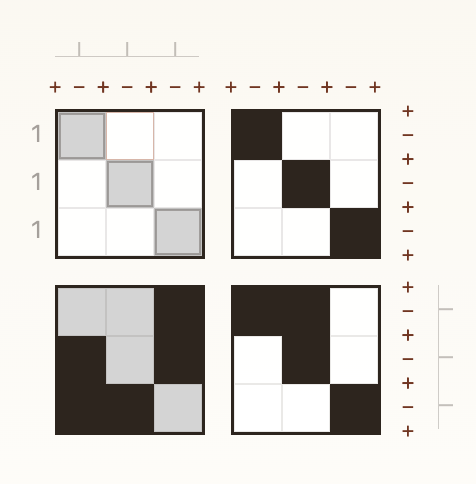
\includegraphics[width=\linewidth]{figures/summer-winter-block.png}
    {\footnotesize Compact block draft}
  \end{minipage}
  \hfill
  \begin{minipage}[t]{0.62\textwidth}
    \centering
    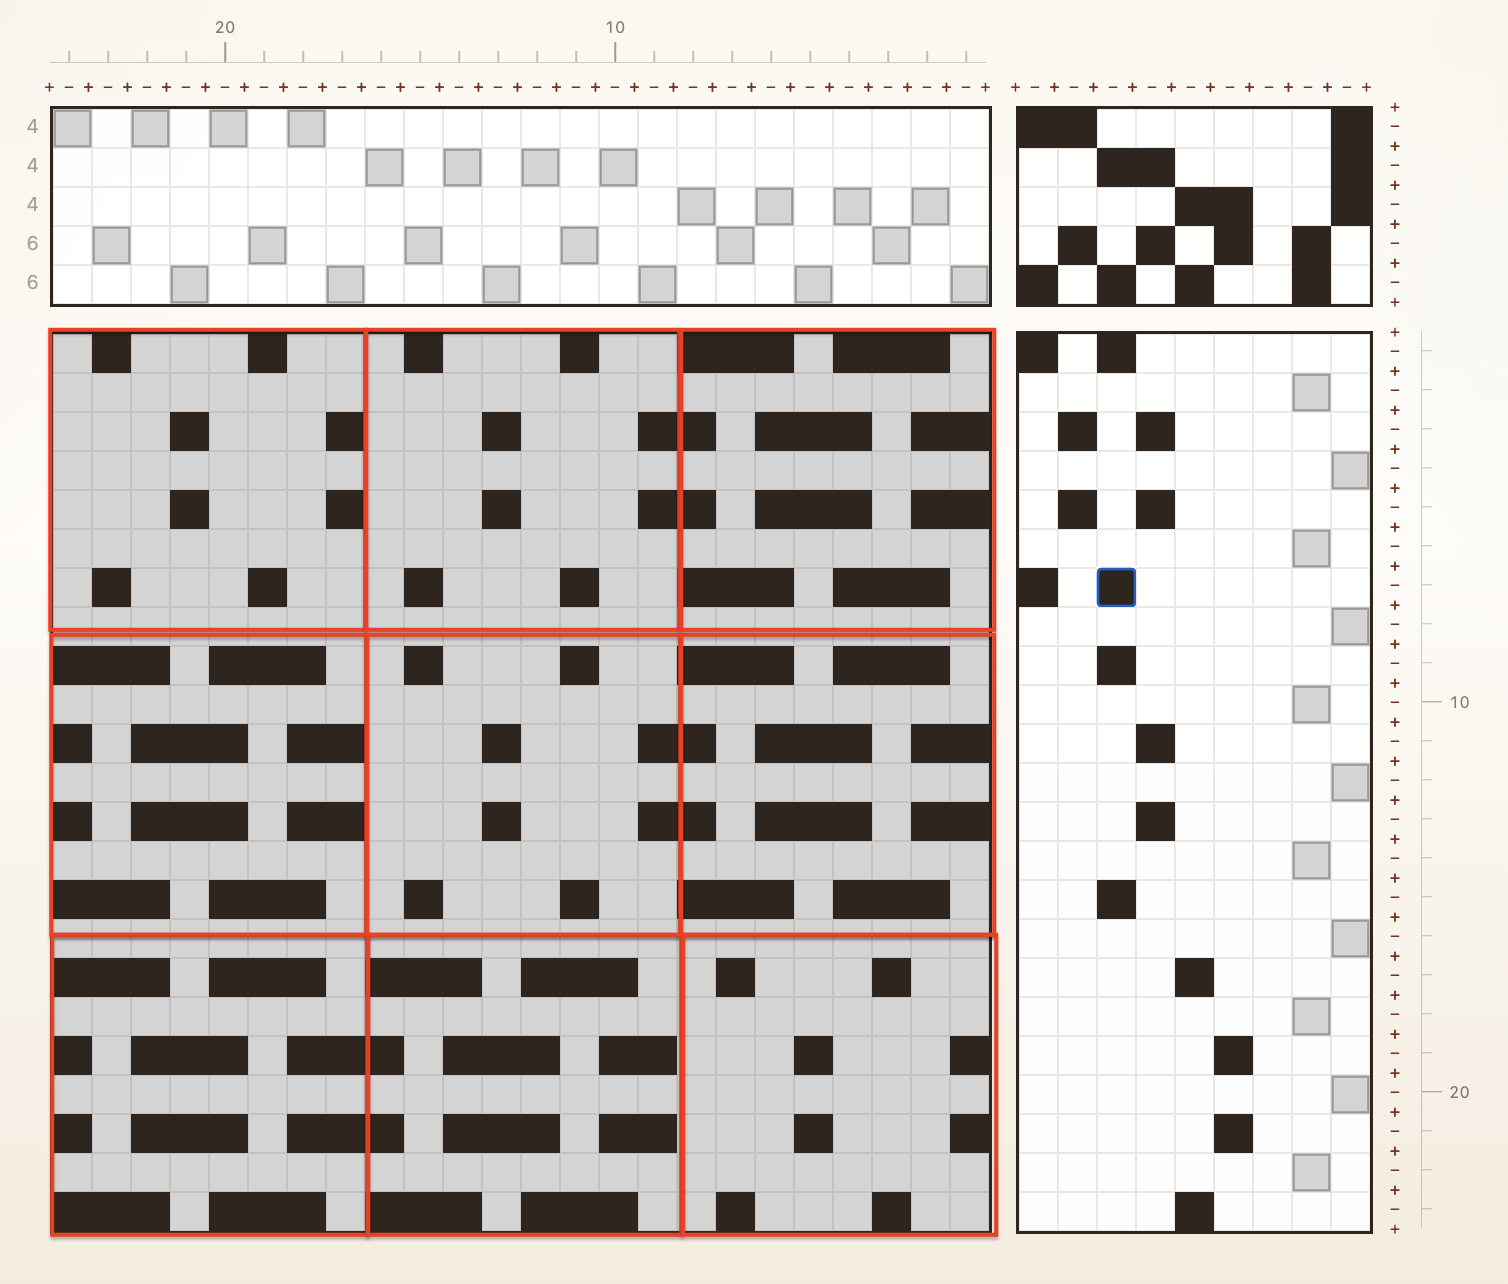
\includegraphics[width=\linewidth]{figures/summer-winter-expanded-annotated.png}
    {\footnotesize Expanded shaft draft}
  \end{minipage}
\end{center}

In the block view, dark means the block is in its default state. Light means
that block group is lifted. Individual cells in the block draft correspond to blocks in the fabric. Removing all background picks and warp threads (shafts 1 and 2, and every other pick) will result in the block pattern draft with duplicate rows and columns. 


\end{document}
